\documentclass[12pt]{article}

\usepackage{amsmath}
\usepackage{amsfonts}
\usepackage{amssymb}
\usepackage{graphicx}
\usepackage[center]{caption}
\usepackage{mathtools}
\usepackage{lipsum}
\usepackage{stackengine}
\usepackage{fancyhdr}
\usepackage{caption}
\usepackage{tikz}
\usetikzlibrary{shapes.geometric, arrows}
\usepackage{float}
\usepackage[a4paper,left=1in,right=1in,top=1in,bottom=1in,footskip=.25in]{geometry}
\usepackage{etoolbox}
\usepackage[nottoc]{tocbibind}
\usepackage{tabu}
\usepackage{enumitem,kantlipsum}
\usepackage{verbatim}
\usepackage{hyperref}
\begin{document}


\section{Aim}
This test case is for checking the capability of the written Isogeometric analysis code of a 2D Piezoelectric plate under mechanical loading with higher-order NURBS basis functions.
\section{Problem description} \label{2DPPWMLPD}
\emph{Section 7.5.1 in Documentation}\\
A 2D piezoelectric plate subjected to mechanical displacements is considered, as shown in Fig. (\ref{EMLoading}) . The material used is PZT-PIC151 ceramics.

\begin{figure}[H]
	\centering
	\begin{minipage}{.5\textwidth}
		\centering
		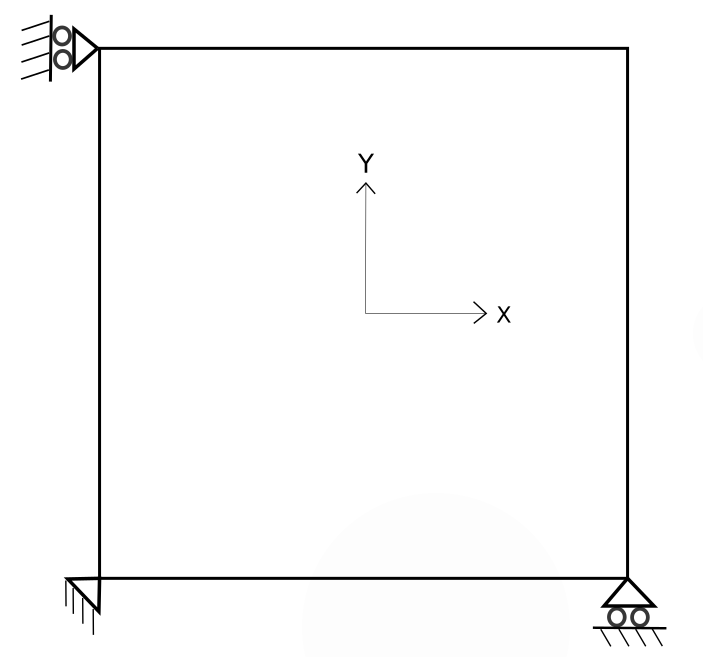
\includegraphics[width=0.8\linewidth]{2DPlate.png}
		\captionof{figure}{2D Piezoelectric Plate}
		\label{2Dplate}
	\end{minipage}%
	\begin{minipage}{.5\textwidth}
		\centering
		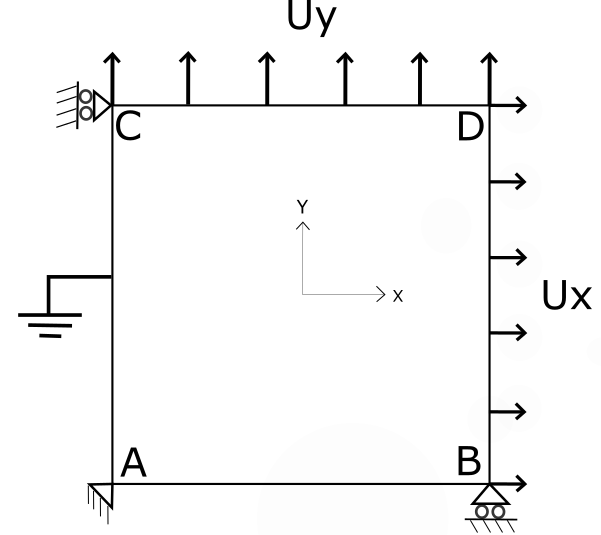
\includegraphics[width=1\linewidth]{Grounded.png}
		\captionof{figure}{2D Piezoelectric Plate with loading}
		\label{EMLoading}
	\end{minipage}
\end{figure}
The movement of the bottom edge AB and left edge AC of 2D piezoelectric plate is fixed in y-direction and x-direction respectively, as shown in figure(\ref{EMLoading}).
The top edge CD is grounded (Electric potential $\Phi = 0$), and a displacement load of 100 nm (1e-4 mm) is applied on the right edge BD. The results for the multiple elements with higher-order NURBS basis functions are discussed in the below
section. \\
In the present load case, a 3rd order basis functions in $\xi$ direction and 4th order basis functions in $\eta$ direction are considered.\\

\newpage

\section{How to run the Program}
\begin{enumerate}[leftmargin=*]
	\item The code is written in python and external libraries numpy, matplotlib.pyplot, sys, path from pathlib and math are used.
	\item Please use any environment which will compile python programs
	\item Place all the files in a single folder.
	\item A file named Input.py can be edited to change the dimensions of the plate. User can change Length, Height and Thickness of the plate. \\(The results discussed below are for Length = 10 mm, Height = 10 mm and Thickness = 1 mm) \\
	\textbf{Also, user can change the degree (p,q) and number of control points (ncpxi,ncpeta) of the curve in each direction.}\\
	The results discussed are for degree (p=2, q=3) and control points (ncpxi=4, ncpeta=5)
	\begin{figure}[H]
		\begin{center}
			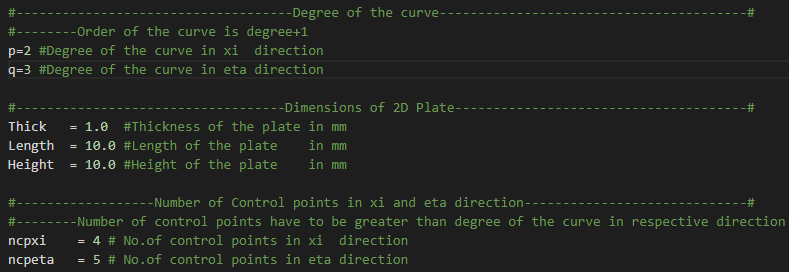
\includegraphics[scale=0.8]{Manual_3parameters.png} 
		\end{center}	
	\end{figure}
	\textbf{Note:} Number of control points have to be greater than degree of the basis functions in respective direction.
	\item Before you run the file, please make sure that the working directory is same as the folder  which
	Consists the Program.
	\item Use command  $>>>$ python Main\_Program.py to run the program.
	\item The contour plots will be saved in the folder \textbf{Results.}
	\item A "log.txt" file is created in the same folder which contains the values of the results plotted.
	
	
\end{enumerate}

\newpage

\section{Results and discussions}
\emph{Section 7.5.3 in Documentation}\\

The displacement (U) values and potential (EPOT) values generated with higher-order NURBS basis functions with more number of control points are compared with the results from 6 elements case.
More control points are used for results only to differentiate between 2nd and higher-order basis functions.
\\
Figure(\ref{EM23U1_IGA_1}) and Figure(\ref{HEM12U1_IGA}) show the displacement (U1) values of the 2nd order NURBS surface and higher-order NURBS surface at 100 \% loading in x-direction respectively. \\
\begin{figure}[H]
	\centering
	\begin{minipage}{.5\textwidth}
		\centering
		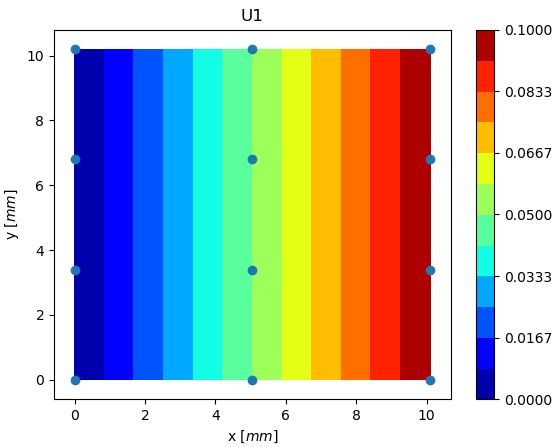
\includegraphics[width=1\linewidth]{EM23U1_IGA.png}
		\captionof{figure}{IGA Piezoelectric Element:U1
			\\\textbf{2nd order NURBS surface}}
		\label{EM23U1_IGA_1}
	\end{minipage}%
	\begin{minipage}{.5\textwidth}
		\centering
		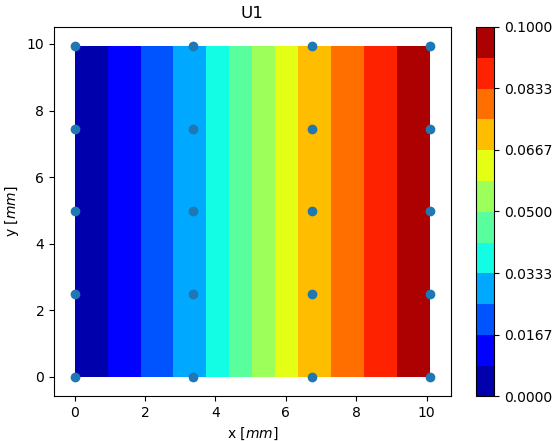
\includegraphics[width=1\linewidth]{HEM12U1_IGA.png}
		\captionof{figure}{IGA Piezoelectric Element:U1\\ \textbf{Higher-order NURBS surface}}
		\label{HEM12U1_IGA}
	\end{minipage}
\end{figure}
\noindent
Figure(\ref{EM23U2_IGA_1}) and Figure(\ref{HEM12U2_IGA}) show the displacement (U2) values of the 2nd order NURBS surface and higher-order NURBS surface at 100 \% loading in the y-direction respectively. \\

\begin{figure}[H]
	\centering
	\begin{minipage}{.5\textwidth}
		\centering
		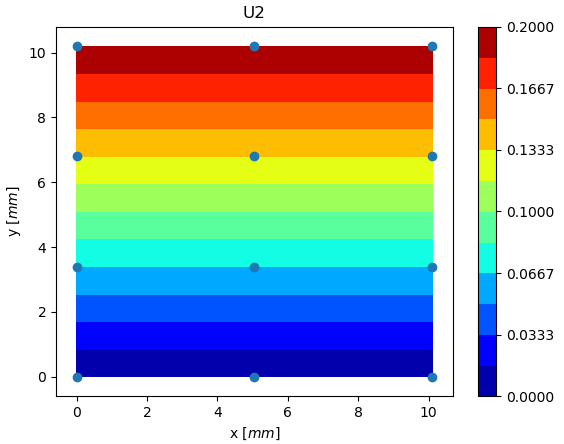
\includegraphics[width=1\linewidth]{EM23U2_IGA.png}
		\captionof{figure}{IGA Piezoelectric Element:U2
			\\\textbf{2nd order NURBS surface}}
		\label{EM23U2_IGA_1}
	\end{minipage}%
	\begin{minipage}{.5\textwidth}
		\centering
		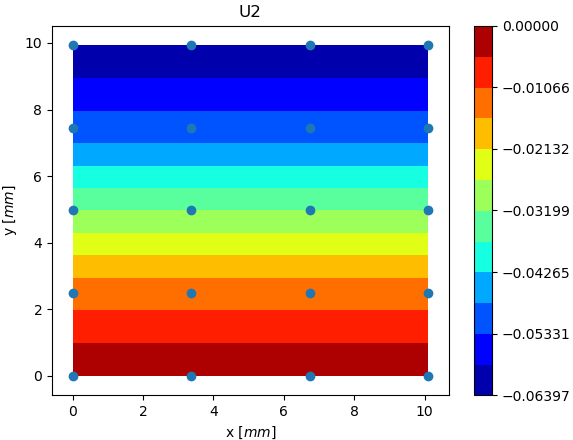
\includegraphics[width=1\linewidth]{HEM12U2_IGA.png}
		\captionof{figure}{IGA Piezoelectric Element:U2\\ \textbf{Higher-order NURBS surface}}
		\label{HEM12U2_IGA}
	\end{minipage}
\end{figure}

Figure(\ref{EM23EPOT_IGA_1}) and Figure(\ref{HEM12EPOT_IGA}) show the Electrical potential (EPOT) values of the 2nd order NURBS surface and higher-order NURBS surface at 100 \% loading respectively. \\
\begin{figure}[H]
	\centering
	\begin{minipage}{.5\textwidth}
		\centering
		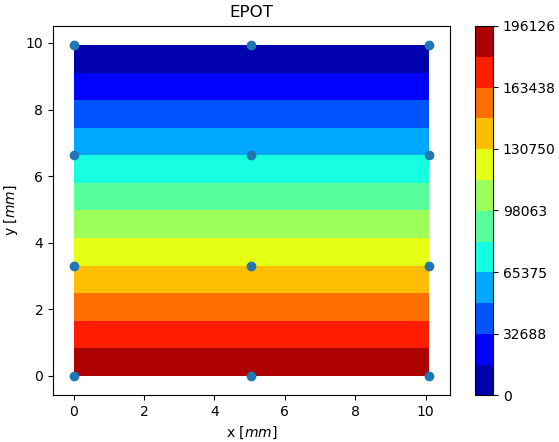
\includegraphics[width=1\linewidth]{EM23EPOT_IGA.png}
		\captionof{figure}{IGA Piezoelectric Element:EPOT
			\\\textbf{2nd order NURBS surface}}
		\label{EM23EPOT_IGA_1}
	\end{minipage}%
	\begin{minipage}{.5\textwidth}
		\centering
		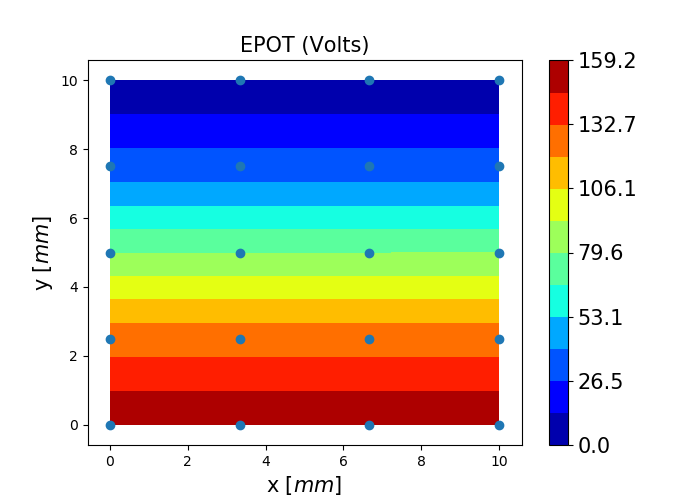
\includegraphics[width=1\linewidth]{HEM12EPOT_IGA.png}
		\captionof{figure}{IGA Piezoelectric Element:EPOT\\ \textbf{Higher-order NURBS surface}}
		\label{HEM12EPOT_IGA}
	\end{minipage}
\end{figure}


\end{document}